\subsubsection{mRNA:ncRNA avoidance}
Recently, Umu et al \cite{Umu2016-zq} found that in bacteria and the archaea, the strength of interactions between mRNAs and non-coding RNAs (ncRNAs) anti-correlate with protein levels. These signals are particularly obvious at the translation initiation site, suggesting that there is an avoidance of inappropriate interactions for highly expressed proteins. However, from a large pool of mRNA and ncRNA, a complete avoidance of interactions is unlikely and a trade off exists between interactions and protein expression. Further, it is suggested that compartmentalisation should minimise these cross talk interactions in eukaryotes. Compartmentalisation has been a topic of considerable research and is linked with noise filtering in gene expression and cellular feedback process \cite{rao2002control, stoeger2016passive, banani2017biomolecular, dong2017shaping}. We now outline in brief, the necessary background to understand the computation of RNA interactions and mRNA:ncRNA avoidance.


\paragraph{Unpairing of bases and accessibility}
McCaskill’s equations \ref{eqn:mcc_restr_part} and \ref{eqn:mcc_full} for the partition function can also be `inverted' to find the probability that $[i^{th}, j^{th}]$ nucleotides are unpaired in the given ensemble. The energy required to unpair the nucleotides is called accessibility or opening energy. If $\kappa \subseteq \Xi$ is the set of all structures $s$ where $[i^{th}, j^{th}]$ nucleotides are unpaired, then the accessibility is given by :

\begin{equation}
\begin{aligned}
    E_{accessibility} &= E_{s \in \kappa} - E_{s \in \Xi}\\
    E_{accessibility} &= -\frac{1}{\beta}\ln{\frac{Z_{unpaired}}{Z}}
\end{aligned}
\end{equation}

The term $\frac{Z_{unpaired}}{Z} = p_u$ is the probability that $[i^{th}, j^{th}]$  nucleotides  are unpaired \cite{Bernhart2011-cc}. Since the pair $i,j$ may or may not be enclosed by a base pair $k,l$ $\ni$ $\forall$ $k,l :$ $ k < i  < j < l$ (Figure \ref{fig:part_fun_decomp}), this probability can be computed by McCaskill approach \cite{Bernhart2011-cc}. Accessibility prediction forms the basis of RNA:RNA interactions. 



\begin{figure}[htbp!]
\center
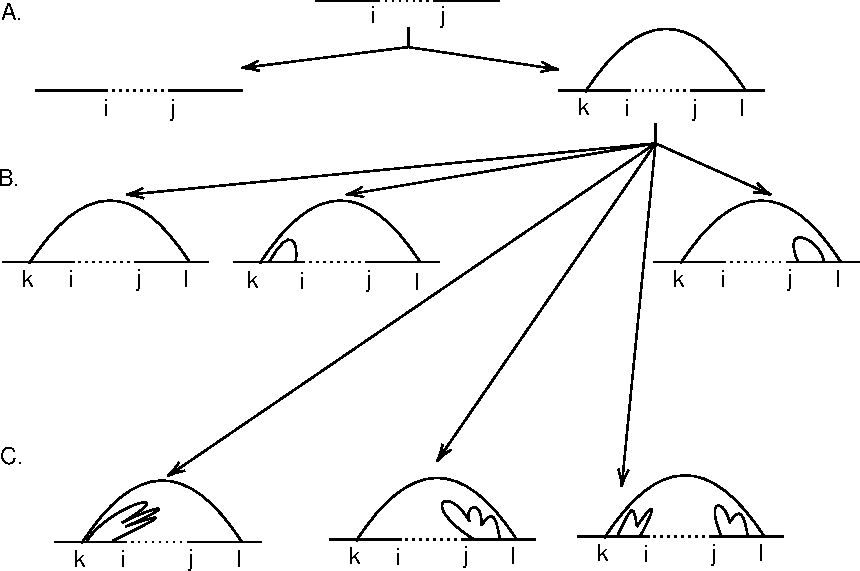
\includegraphics[width=1\textwidth]{chapters/Introduction/Figures/accs.pdf}
\caption[Decomposition of partition function to calculate unpairing probability of the region $(i,j)$ in a nucleotide sequence.]{\textbf{Decomposition of partition function to calculate unpairing probability of the region $[i,j]$ in a nucleotide sequence. (A)}  The interval [i,j] may either be enclosed by pair [k,l] (right) or may be open (left). \textbf{(B)} The enclosed pair may or may not contain an hairpin or \textbf{(C)} multiloops. The partition function $Z_{unpaired}$ is a sum of all these contributions.  Figure adapted from Bernhart \textit{et al.}, (2011)}%the List of Figures because of the *}
\label{fig:part_fun_decomp}
\end{figure}


% The exact equation to compute this probability and the accessibility in $\mathcal{O}(n^{3})$ time is given by Bernhart \textit{et al.}  with an algorithmic implementation in RNAplfold of ViennaRNA suite \cite{Lorenz2011-rg}. Accessibility prediction forms the basis of RNA:RNA interactions. 


\paragraph{RNA:RNA interactions} \label{subsec:rna_interac}
For two RNA molecules to interact and pair, most computational tools assume that this is  a two step process\textemdash unfolding of the RNA molecules at the target sites, followed by an actual interaction (hybridisation) \cite{Muckstein2006-ys}.
Thus, the total binding energy $\Delta G$ is the sum of the accessibility of the target site of the longer RNA molecule $\Delta G_{unpaired}$ and the subsequent interaction between the unfolded region of the interacting molecules $\Delta G_{int}$. $\Delta G_{unpaired}$ is computed by equation $1.8$, where as $\Delta G_{int}$ is computed through equation \ref{eqn:free_en} by replacing $Z$ with $Z_{int}$. For an interaction between nucleotides $[i, j]$ and $[i^*, j*]$ the partition function $Z_{int}$ is given by \cite{Muckstein2006-ys} (Figure \ref{fig:part_fun_interac}):





\begin{equation}
\begin{aligned}
    Z_{int} &= p_u[i,j] \sum_{i^*>j*} Z^I[i,j,i^*,j^*] \\
    where, \\
    Z^I[i,j,i^*,j^*] &= \sum_{\substack{i<k<j\\
    j*<k^*<i^*}} Z^1[i,k,i^*,k^*] e^{E_I(i,k,i^*,k^*)}
\end{aligned}
\end{equation}

with $E_I(i,k,i^*,k^*)$ as the free energy of the interior loop enclosed by $(i,k)$ and $(i^*,k^*)$ and $Z^1[i,k,i^*,k^*]$ contains at least one substructure between $(i,k)$ and $(i^*,k^*)$. 

\begin{wrapfigure}{r}{0.5\textwidth}
  \begin{center}
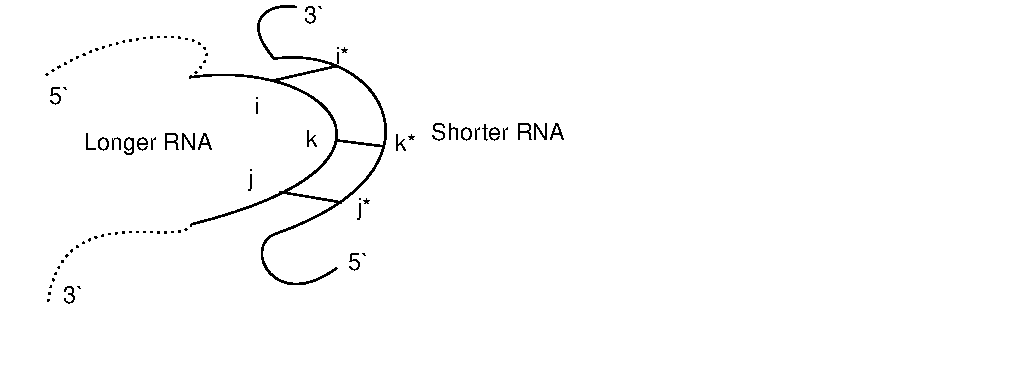
\includegraphics[width=0.7\textwidth]{chapters/Introduction/Figures/interac.pdf}
\caption[RNA:RNA interaction and notations used for partition function.]{\textbf{RNA:RNA interaction and notations used for partition function.} Full shape of longer RNA is not shown. The nucleotides between $[i,j]$ and $[i^*,j^*]$ may contain mismatches. Figure adapted from Muckstein \textit{et al.}, (2006). }%the List of Figures because of the *}
\label{fig:part_fun_interac}
  \end{center}
\end{wrapfigure}

The RNA:RNA interaction prediction mechanisms are still being actively refined because many RNA:RNA interactions have important regulatory functions. For example, in eukaryotes, microRNAs can reduce the levels of mRNAs by interacting with the $3^{\prime}$UTRs of the mRNA targets \cite{catalanotto2016microrna, valencia2006control}.




